%\headrulewidth% file pasantia.tex
% Archivo pasantia.tex
% Documento maestro que incluye todos los paquetes necesarios para el documento
% principal.

% Documento obtenido por un sinfin de iteraciones de administradores del LDC
% Estructura actual hecha por:
% Jairo Lopez <jairo@ldc.usb.ve>
% Actualizado ligeramente por:
% Alexander Tough 

\documentclass[oneside,12pt,letterpaper,openany]{report}
\tolerance=1000  
\hbadness=10000  
\raggedbottom

% Paquetes para manejar graficos
\usepackage{epsf}
\usepackage{float}
\usepackage[pdftex]{graphicx}
\usepackage{epsfig}
% Simbolos matematicos
\usepackage{latexsym,amssymb}
% Paquetes para presentar una tesis decente.
\usepackage{setspace,cite} % Doble espacio para texto, espacio singular para
                           % los caption y pie de pagina

% Paquetes no utilizados para citas
%\usepackage{mcite} 
%\usepackage{draft} 

\usepackage{wrapfig}
\usepackage{alltt}

% Acentos 
\usepackage[spanish,activeacute]{babel}
\usepackage[spanish]{translator}
\usepackage[utf8]{inputenc}
\usepackage{color, xcolor, colortbl}
\usepackage{multirow}
\usepackage{subfig}
\usepackage[OT1]{fontenc}
\usepackage{tocbibind}
\usepackage{anysize}
\usepackage{listings} 

% Para poder tener texto asiatico
%\usepackage{CJK}

% Opciones para los glosarios
\usepackage[style=altlist,toc,numberline,acronym]{glossaries}
\usepackage{url}
\usepackage{amsthm}
\usepackage{amsmath}
\usepackage{fancyhdr} % Necesario para los encabezados
\usepackage{fancyvrb}
\usepackage{makeidx} % En caso de necesitar indices.
\makeindex  % Necesitado para los indices

% Definiciones para definicions, teoremas y lemas
\theoremstyle{definition} \newtheorem{definicion}{Definici\'{o}n}
\theoremstyle{plain} \newtheorem{teorema}{Teorema}
\theoremstyle{plain} \newtheorem{lema}{Lema}

% Para la creacion de los pdfs
\usepackage{hyperref}

% Para resolver el lio del Unicode para la informacion de los PDFs
% En pdftitle coloca el nombre de su proyecto de grado/pasantia.
% En pdfauthor coloca su nombre.
\hypersetup{
    pdftitle = {TITULO DE LA PASANTIA},
    pdfauthor={AUTOR},
    colorlinks,
    citecolor=black,
    filecolor=black,
    linkcolor=black,
    urlcolor=black,
    backref,
    pdftex
}

% Crea el glosario
\makeglossaries




% Para crear la hoja escaneada de las firmas
\usepackage[absolute]{textpos}

% Pone los nombres y las opciones para mostrar los codigos fuentes
\lstset{language=C, breaklines=true, frame=single, showstringspaces=false,
        showtabs=false, numbers=left, keywordstyle=\color{black},
        basicstyle=\footnotesize, captionpos=b }
\renewcommand{\lstlistingname}{C\'{o}digo fuente}
\renewcommand{\lstlistlistingname}{\'{I}ndice de c\'{o}digos fuentes}

% Dimensiones de la pagina
\setlength{\headheight}{15pt}
\marginsize{3cm}{2cm}{2cm}{2cm}

% Se pueden omitir para que no compile ciertos capitulos.
\includeonly{header, intro, ssimilar, herramienta, resultados, conclusiones}

%%%%%%%%%%%%%%%%%%%%%%%%%%%%%%%%%%%%%%%%%%%%%%%%%%%%%%%%%%%%%%%%%%%%%%%%%%%
%%%%%%%%%%%%%%%%      end of preamble and start of document     %%%%%%%%%%%
%%%%%%%%%%%%%%%%%%%%%%%%%%%%%%%%%%%%%%%%%%%%%%%%%%%%%%%%%%%%%%%%%%%%%%%%%%%
\begin{document}

% Pagina de titulo
% Pagina de titulo
\begin{titlepage}
\begin{center}

% Upper part (aqui ya esta incluido el logo de la USB).

\includegraphics[scale=0.5,type=png,ext=.png,read=.png]{figures/cebolla} \\

% Encabezado
\textsc {\large UNIVERSIDAD SIM'ON BOL'IVAR} \\
\textsc{\bfseries DECANATO DE ESTUDIOS PROFESIONALES\\
COORDINACI'ON DE INGENIER'IA DE LA COMPUTACI'ON}

\bigskip
\bigskip
\bigskip
\bigskip
\bigskip
\bigskip
\bigskip
\bigskip
\bigskip

% Title/Titulo
% Aqui ponga el nombre de su proyecto de grado/pasantia larga
\textsc{\bfseries CONFIGURACI'ON DE SAP ERP PARA UN MODELO DE INDUSTRIA DE CONSUMO MASIVO (CPG)}

\bigskip
\bigskip
\bigskip
\bigskip
\bigskip

% Author and supervisor/Autor y tutor
\begin{minipage}{\textwidth}
\centering
Por: \\
JULIO DE ABREU MOLINA \\

\bigskip
\bigskip
\bigskip

Realizado con la asesor'ia de: \\
KENYER DOM'INGUEZ
\end{minipage}

\bigskip
\bigskip
\bigskip
\bigskip
\bigskip
\bigskip
\bigskip
\bigskip
\bigskip

% Bottom half
{PASANT\'IA LARGA \\ Presentado ante la Ilustre Universidad Sim'on Bol'ivar \\
como requisito parcial para optar al t'itulo de \\ Ingeniero en Computaci'on} \\

\bigskip
\bigskip
\vfill

% Date/Fecha 
{\large \bfseries Sartenejas, febrero del 2014}

\end{center}
\end{titlepage}


% Pagina de acta final (vacio)
% Pagina del acta final
\begin{titlepage}
\begin{center}

% Upper part

\includegraphics[scale=0.5,type=png,ext=.png,read=.png]{figures/cebolla} \\

\textsc {\large UNIVERSIDAD SIM'ON BOL'IVAR} \\
\textsc{DECANATO DE ESTUDIOS PROFESIONALES\\
COORDINACI'ON DE INGENIER'IA DE LA COMPUTACI'ON}

\bigskip
\bigskip
\bigskip
\bigskip
\bigskip
\bigskip

% Title
\textsc{ACTA FINAL PASANT\'IA LARGA}

\bigskip
\bigskip

% Aqui coloca el nombre de su proyecto de grado/pasantia larga.
\textsc{\bfseries CONFIGURACI'ON DE SAP ERP PARA UN MODELO DE INDUSTRIA DE CONSUMO MASIVO (CPG)}

\bigskip
\bigskip
\bigskip
\bigskip

\begin{minipage}{\textwidth}
\centering
Presentado por: \\
% Aqui coloca su nombre.
\textsc{\bfseries JULIO DE ABREU MOLINA} \\

\bigskip
\bigskip
\bigskip
\bigskip

Esta Pasant\'ia Larga ha sido aprobado por el siguiente jurado examinador: \\

\bigskip
\bigskip

% Despues de cada line coloca el (los) nombre(s) de
% cada uno de los integrantes del jurado.
\line(1,0){200} \\
KENYER DOM'INGUEZ\\

\bigskip
\bigskip

\line(1,0){200} \\
PROFESOR 2 \\

\bigskip
\bigskip

\line(1,0){200} \\
ANA CECILIA GARCIA REVER'ON \\
\end{minipage}

\bigskip
\bigskip
\vfill

% Date/Fecha
{\large \bfseries Sartenejas, FECHA (dd/mm/aa)}

\end{center}
\end{titlepage}


\setcounter{secnumdepth}{3}
\setcounter{tocdepth}{4}

% Define encabezado numeros romanos y como se separan los captiulos y las
% secciones
\addtolength{\headheight}{3pt}
\pagenumbering{roman}
\pagestyle{fancyplain}

\renewcommand{\chaptermark}[1]{\markboth{\chaptername\ \thechapter:\,\ #1}{}}
\renewcommand{\sectionmark}[1]{\markright{\thesection\,\ #1}}

\onehalfspacing

\lhead{}
\chead{}
\rhead{}
\renewcommand{\headrulewidth}{0.0pt}
\lfoot{}
\cfoot{\fancyplain{}{\thepage}}
\rfoot{}


% Pagina de resumen
\setcounter{page}{4}
\begin{center}
	{\bf Resumen}
\end{center}	

\indent El presente documento abarca los procesos de an'alisis y configuraci'on del m'odulo de Ventas y Distribuci'on \textbf{(SD)} de \textbf{SAP} para un modelo de empresas de bebidas de consumo masivo, con la finalidad de que una empresa de este rubro pueda contar con un sistema que le permita gestionar la venta y distribuci'on de todos los productos que elabore.
\newline
\newline
\indent Durante este proyecto se llev'o a cabo un an'alisis del modelo de negocio de una empresa de bebidas de consumo masivo, para poder conocer c'omo es el proceso de Ventas y Distribuci'on que esta ejecuta. Este proceso permiti'o el dise\~no y la posterior configuraci'on del m'odulo \textbf{SD} de \textbf{SAP}, el cual est'a adaptado a las necesidades de dicha empresa.
\newline
\newline
\indent El proyecto se llev'o a cabo de forma exitosa, obteni'endose un m'odulo de Ventas adaptado a las necesidades de un modelo de empresas de bebidas. Para su realizaci'on, se emple'o la metodolog'ia \textbf{ASAP (Ascendant SAP)}, y el software \textbf{SAP}. Para los elementos no configurables, tuvieron que ser programados a trav'es del lenguaje \textbf{ABAP/4}, y para su dise\~no previo se realiz'o un diagrama de actividades con notaci'on \textbf{UML 2.0}.

\newpage


% Pagina de dedicatoria (opcional)
\setcounter{page}{5}

\vspace*{8cm} 
\pdfbookmark[0]{Dedication}{dedication} % Sets a PDF bookmark for the dedication
\begin{center} 
\large DEDICATORIA
\end{center}
\newpage


% Pagina de agradecimientos (opcional)
\setcounter{page}{6}

\chapter*{Agradecimientos
\markboth{Agradecimientos}{Agradecimientos}}
AQU\'I VAN LOS AGRADECIMIENTOS.







% Crea la tabla de contenidos
\tableofcontents

% Crea la lista de cuadros
\listoftables

% Crea la lista de figuras
\listoffigures
% Incluye el glosario
\newacronym{SQL}{SQL}{Structured Query Language $H$}

\newacronym{asie-h}{asie-H}{proceso autosimilar con par\'{a}metro autosimilar
$H$ e incrementos estacionarios}

\newacronym{aas-h}{aas-H}{proceso asint\'{o}ticamente autosimilar con
par\'{a}metro autosimilar $H$}

\printglossary

% Crea la lista de codigos fuentes
%\lstlistoflistings

\clearpage

% Define encabezado en numeros arabicos  
\pagenumbering{arabic}

\fancyhf{} % Redefine el encabezado 
\lhead{}
\chead{}
\rhead{\fancyplain{}{\thepage}}
\renewcommand{\headrulewidth}{0.0pt}
\lfoot{}
\cfoot{}
\rfoot{}

\doublespacing


% Incluye los archivos deseados - El contenido de
% su proyecto de grado/pasantia larga.
 \addcontentsline{toc}{chapter}{Introducci\'on}

% Titulo de la introduccion.
\begin{center}
	{\bf Introducci\'on} \label{chap:intro}
\end{center}

% Contenido de la introduccion.

\label{sect:motivacion}
%Puedes quitar esto(es opcional)
\vspace{5 mm}

AQU\'I VA EL CONTENIDO DE ANTECEDENTES. 

%Puedes quitar esto(es opcional)
\vspace{5 mm}

\label{sect:justificacion}
%Puedes quitar esto(es opcional)
\vspace{5 mm}

AQU\'I VA EL CONTENIDO DE LA JUSTIFICACI\'ON.
%Puedes quitar esto(es opcional)
\vspace{5 mm}

En la Universidad de Tohoku de Sendai, Jap'on, en el laboratorio Kinoshita de
la facultad de Ciencias de la Computaci'on, se tiene un {\it framework} con el
cual han creado un {\it Active Information Resource} (AIR) - {\it Network
Management System} (NMS) \cite{kinoshitaNMSAIR} para gestionar las redes de
computadoras. Mediante el lenguaje de programaci'on orientado a agentes
basado en Java, DASH ({\it Repository-based Agent Framework}) y su ambiente
de dise~no interactivo IDEA ({\it Interactive Design Environment}), la idea
final es que la red y los elementos que la componen se pueda auto-gestionar
mediante los agentes instalados en los elementos \cite{545112}, sin la
necesidad de tener un administrador. El objectivo es identificar y solucionar
los problemas de la red en tiempo real \cite{AbarAK04} \cite{KonnoAIK07}.

%Puedes quitar esto(es opcional)
\vspace{5 mm}


\label{sect:planteamiento}
%Puedes quitar esto(es opcional)
\vspace{5 mm}

AQU\'I VA EL CONTENIDO DEL PLANTEAMIENTO DEL PROBLEMA.

En los 'ultimos a~nos ha habido un gran inter'es por determinar si los nuevos
modelos basados en la autosimilaridad y la dependencia de largo alcance pueden
ser utilizados para la detecci'on de anomal'ias en las redes de datos
\cite{5475821}. Entre las anomal'ias m'as destacadas se encuentran las de
ataques de denegaci'on de servicio y su ampliaci'on: el llamado ataque
distribuido de denegaci'on de servicio \cite{mingliddos} \cite{xiang:292}.

En el trabajo de \cite{mingliddos} se utiliz'o, con buenos resultados, el
c'alculo del grado de autosimilaridad para detectar anomal'ias en la red. Se
realiz'o una implementaci'on para un {\it framework} de autogesti'on de redes
desarrollado en el laboratorio Kinoshita de la Universidad de Tohoku. Como se
explica en la pr'oxima secci'on la idea del proyecto de grado fue mejorar esta
implementaci'on.

%Puedes quitar esto(es opcional)
\vspace{5 mm}

\label{sect:objetivo_general}
%Puedes quitar esto(es opcional)
\vspace{5 mm}

\indent El objetivo principal del proyecto es la de la implementaci'on de una soluci'on \emph{SAP SD} en una empresa de bebidas de consumo masivo \emph{SSA CPG} para gestionar los procedimientos comerciales. 


%Puedes quitar esto(es opcional)
\vspace{5 mm}

\label{sect:objetivos_especificos}
%Puedes quitar esto(es opcional)
\vspace{5 mm}

\begin{enumerate}
\item Adquirir los conocimientos de la Metodología Ascendant SAP y el funcionamiento del Sistema SAP en la funcionalidad Ventas y Distribuci'on (SD).

\item Analizar los procesos de Ventas y Distribuci'on con las funcionalidades SAP que los soportan. Adquirir los conocimientos generales del negocio, procesos y visi'on global de la soluci'on SAP a implantar.

\item Configurar los campos del sistema a implantar para el m'odulo SD acorde a las necesidades del cliente, hacer los desarrollos necesarios y probar las funcionalidades SAP ERP SD que soportan los procesos comerciales.

\item Preparar los datos y el sistema, realizar la demostraci'on y documentar los resultados correspondientes al m'odulo SD, para comprobar el funcionamiento y configuraci'on del m'odulo de manera individual y en relaci'on con otros m'odulos implicados del sistema.

\end{enumerate}

La implementaci'on deber'a tomar como entrada una traza creada por la librer'ia
{\tt libpcap}\footnote{Esta librer'ia provee una interfaz de alto nivel para la
captura y manipulaci'on de los paquetes a bajo nivel pudiendo manipular todos 
los paquetes, incluidos aquellos destinados a otros nodos de red. La librer'ia
se encuentra disponible en \url{http://www.tcpdump.org}.} y poder
crear f'acilmente una serie de tiempo para la estimaci'on del par'ametro de
Hurst, haciendo flexible la estimaci'on con diferentes series de tiempo creadas
a partir de la misma traza. Como salida, el programa debe graficar los
resultados de las estimaciones del par'ametro de Hurst, incluyendo el cambio del
par'ametro en el tiempo, para as'i poder verificar de forma r'apida los
resultados. 

Una vez validada la estimaci'on del par'ametro de Hurst, se deber'a verificar si
esta estimaci'on puede ser utilizada para detectar las anomal'ias en tiempo
real creadas por un ataque distribuido de denegaci'on de servicio en las trazas
de red.



% Marco Teorico.
\chapter{Entorno Empresarial} \label{chap:empresa}



\section{Descripci'on General} \label{sect:descripcion}
\textbf{International Business Machines (IBM)} es una corporaci'on americana con sede principal en Armonk, New York, USA. Esta corporaci'on a lo largo de los a\~nos se ha encargado de ofrecer soluciones inteligentes a sus clientes. Entre los servicios que ofrece, se pueden mencionar los siguientes:
\begin{itemize}
\item Software: Dentro de los productos que ofrece, se encuentran: Rational, IBM Websphere, Lotus, etc.
\item Hardware
\item Consultor'ia: A trav'es del Departamento de \textbf{Business Global Services (GBS)}, IBM ofrece servicios de consultor'ia a las distintas empresas ofreci'endoles \textbf{SAP} como producto para manejar toda la parte funcional de las mismas.
\end{itemize}

\section{Misi'on} \label{sect:mision}
"Ayudar a nuestros clientes a alcanzar sus metas de negocio provey'endoles servicios y soluciones innovadoras"

\section{Visi'on} \label{sect:vision}
"Se la compa\~n'ia elegida por nuestra innovaci'on, soluciones, productos y servicios. Ser reconocida por la calidad humana y profesional de nuestra gente y por nuestra contribuci'on a la comunidad"

\section{Estructura Organizacional} \label{sect:organizacion}

\section{Ubicaci'on del Pasante}
	Durante el desarrollo del proyecto, el pasante ocup'o el cargo de \textbf{Consultor SAP Junior SD \& ABAP}, perteneciendo al Departamento de  \textbf{Global Business Services (GBS)}. Su jefe Inmediato fue su Tutora Industrial y Gerente del Departamento, la Ing. Ana Cecilia Garc'ia Rever'on. 
% Marco Teorico.
\chapter{Marco te'orico} \label{chap:ssimilar}



Los conceptos claves acerca de lo que es un sistema ERP, SAP, ABAP son los que se presentan en este capítulo.
\newline
\newline
La secci'on ~\ref{sect:erp} presenta las nociones b'asicas acerca de en qu'e consiste un Sistema de Informaci'on ERP. La secci'on 
~\ref{sect:sap} describe un poco lo que es SAP: sus caracter'isticas principales, una  breve historia. Por otro lado, la secci'on ~\ref{sect:abap} explica en que consiste el lenguaje de programaci'on ABAP, sus principales caracter'isticas. 

\section{Sistemas de Informaci'on ERP} \label{sect:erp}

Para entender en qu'e consisten los Sistemas de Informaci'on ERP, para ello habr'a que definir dos conceptos fundamentales: Sistema de Informaci'on, y m'as a'un, Sistemas ERP. 

\subsection{Definiciones} \label{subsect:defprop}

\begin{definicion} \label{def:sisinfo}
	Un Sistema de Informaci'on es un conjunto de componentes capaces de interactuar mutuamente con el objetivo de brindar apoyo a las actividades de una empresa o negocio.

\end{definicion}

\begin{definicion} \label{def:siserp}
Un ERP (Sistema de Planificación de Recursos Empresariales, 'o como se le conoce en Ingl'es: \textbf{Enterprise Resource Planning}), es un sistema que tiene la capacidad de la automatizaci'on e integraci'on de todos los m'odulos de un 'area de negocio. En otras palabras, es capaz de manejar todas las 'areas relacionadas con una empresa de forma automatizada e integrada. 
\newline
\newline
Una caracter'istica fundamental de este tipo de sistemas es que est'a basado en m'odulos. Como consecuencia de ello, el mismo est'a compuesto por un conjunto de softwares o m'odulos. 
\newline
\newline
Para poder tener acceso a los datos que est'an relacionados con cada m'odulo es necesario tener una Base de Datos centralizada, la cual almacena dicha informaci'on. 
\end{definicion}

\section{SAP} \label{sect:sap}

En esta secci'on se ofrece un panorama general acerca de SAP, qu'e es, cu'ales son sus caracter'isticas principales y cu'ales son los m'odulos que lo integra.

\subsection{Definici'on} \label{subsect:defprop}
\textbf{SAP AG} es una empresa de la rama de la Computaci'on que fue fundada por 4 ingenierosque pertenecieron a IBM (\textbf{International Business Machines}), en la ciudad de Walldorf, Alemania, en el a~no de 1972. Por su origen alem'an, las siglas SAP son un acr'onimo de: \textit{Systeme, Anwendungen Produkte in der Datenverarbeitung}, que traducido al castellano significa: \textbf{Sistemas, Aplicaciones y Productos en Procesamiento de Datos}. 
\newline
\newline
El Software principal desarrollado por esta empresa es \textbf{\textit{SAP R/3}} y el cual se encuentra disponible en 28 idiomas. 'Este software es personalizable, utiliza la arquitectura cliente-servidor, es decir, que el cliente envia solicitudes al servidor y 'este a su vez envia una respuesta al cliente. 'Este software fue hecho en el lenguaje de programaci'on \textbf{ABAP/4}. 

\subsection{Caracter'isticas de SAP R/3}
De acuerdo al autor de \cite{SAP01}, las caracter'isticas del software \textbf{SAP R/3} se pueden dividir en diferentes categor'ias, las cuales se mencionan a continuaci'on:

\subsubsection*{Caracter'isticas Generales}
\begin{itemize}
\item Es un software altamente integrado y multifuncional, lo que trae como consecuencia que exista una estrecha relaci'on entre las funciones del mismo.
\item Es una aplicaci'on que trabaja en tiempo real. En otras palabras, las actualizaciones de los datos son efectuadas a trav'es de una conexi'on, y en ese mismo instante.
\end{itemize}
\subsubsection*{Caracter'isticas de Negocio}
\begin{itemize}
\item Este software contiene todas las funcionalidades necesarias para poder llevar a cabo el manejo de un negocio entero. 'Este incorpora una aplicaci'on llamada \textit{Best Industry Practices}, que traducido al espa\~nol quiere decir: \textit{Mejores Practicas de la Industria}, y 'este 'ultimo es adecuado para una amplia gama de industrias y organizaciones.
\item Este programa es capaz de soportar todos los procesos de negocio de la empresa.
\end{itemize}

\subsubsection*{Caracter'isticas de Flexibilidad}
\begin{itemize}
\item Este software es altamente configurable. En otras palabras, se puede adaptar a las necesidades de la empresa que lo utilice y a sus requerimientos. Para ello, se pueden realizar cambios que, dependiendo del n'umero de factores que participen, 'estos tendr'an su grado de complejidad.
\item Es capaz de dar apoyo a empresas que poseen subsidiarias en distintas partes del mundo.
\item Este software es muy utilizado a nivel mundial, dado que est'a disponible en 28 idiomas, y a que posee la capacidad de adaptarse a la moneda, leyes y regulaciones, impuestos para un cierto pa'is, etc.
\end{itemize}

\subsubsection*{Caracter'isticas T'ecnicas}
\begin{itemize}
\item Este software tiene la capacidad de ser portable, dado que es multiplataforma, es decir, soporta cualquier sistema operativo, manejador de Base de Datos, etc.
\item Posee un n'umero m'inimo de redundancia, lo que favorece a la consistencia de los datos almacenados. Adicionalmente, posee un manejador de alta seguridad de los datos, y puede manejar etructuras de datos complejas.
\end{itemize}

\subsubsection*{Otras Caracter'isticas}
\begin{itemize}
\item Tiene la capacidad de manejar la misma informaci'on en cada m'odulo.
\item Posee una 'unica manera de ingreso al sistema. 'Este es a trav'es del \textit{SAP GUI}.
\item Tiene la capacidad de ser escalable, es decir, que est'a preparado para manejar el continuo crecimiento del trabajo sin disminuir la calidad.
\item Tiene una interfaz gr'afica amigable.
\end{itemize}

\subsection{Adaptaci'on del Software a las Empresas}
Para poder realizar la adaptaci'on de SAP a las necesidades de una empresa en particular, est'an un conjunto de herramientas y utilidades destinado a ello. Para esto, se requiere de un conjunto de consultores, un equipo de proyecto y personal de Tecnolog'ia de la Informaci'on (IT), quienes ser'an los encargados de efectuar dicha adaptaci'on. 
\newline
\newline
Este proceso se puede realizar a trav'es de dos m'etodos, los cuales se listan a continuaci'on:

\begin{itemize}
\item \textbf{Cambios en la Configuraci'on:} Aqu'i son modificadas las tablas relacionadas con los distintos m'odulos para poder realizar la adaptaci'on.
\item \textbf{Programaci'on en el Lenguaje ABAP/4:} Esto implica modificar programas ya existentes en \textbf{SAP R/3} o crear programas nuevos.
\end{itemize}

\subsection{M'odulos de SAP R/3}
Debido a que SAP es un ERP, luego, SAP est'a dividido en diferentes m'odulos, con el fin de poder abarcar cada 'area de una empresa. Estos m'odulos son los que se listan a continuaci'on:

\begin{enumerate}
\item Asset Management (Manejo de Aplicaciones - AM)
\item Financials (Finanzas - FI)
\item Controlling (Control - CO)
\item Human Resources (Recursos Humanos - HR)
\item Plant Maintenance (Mantenimiento de Planta - PM)
\item Production Planning (Planificaci'on de la Producci'on - PP)
\item Project System (Sistema de Proyectos - PS)
\item Quality Management (Manejo de Calidad -QM)
\item Sales and Distribution (Ventas y Distribuci'on - SD)
\item Materials Management (Manejo de Materiales - MM)
\item Services Management (Manejo de Servicios - SM)
\item Industry Specific Solutions (Soluciones Espec'ificas para la Industria - IS)
\item Business Workflow (Flujo de trabajo del Negocio - WF)
\item Basis (Incluye el lenguaje de programaci'on \textbf{ABAP 4} - BC).

\end{enumerate}

\section{M'odulo de Ventas y Distribuci'on (SD)} \label{sect:sd}

El \textbf{M'odulo de Ventas y Distribuci'on} (Sales and Distribution como es conocido en ingl'es) es un sub-sistema perteneciente a SAP, el cual se encarga de prestar apoyo a las distintas empresas en el 'area de las Ventas y distribuci'on de productos y/o servicios. 
\newline
\newline
Este m'odulo ayuda a las compa\~n'ias a establecer un precio para sus productos, chequear 'ordenes de ventas que se mantienen abiertas, a tomar previsiones para necesidades futuras, etc. Adicionalmente, ayuda a dar mayor control a las actividades relacionadas con el 'area de ventas: desde el momento en que ocurre un pedido de alg'un(algunos) producto(s) y/o servicio(s) hasta su posterior entrega.



\subsection{Herramientas Principales}
\subsubsection{Manejo de Precios e Impuestos}
A trav'es de esta herramienta, el m'odulo puede evaluar los precios que son colocados a los productos o servicios de acuerdo a unas condiciones establecidas previamente. 
\subsubsection{Chequeo de Disponibilidad}
Con esta herramienta, el m'odulo puede evaluar la disponibilidad de un producto para un almac'en especificado.
\subsubsection{Manejo de Cr'edito}
Con esta herramienta es posible establecer l'imites de cr'edito para un cliente durante el proceso de ventas en el cual se encuentra envuelto.
\subsubsection{Facturaci'on}
Una vez que una Orden de Ventas es creada, se utiliza esta herramienta para crear la(s) factura(s) asociadas.
\subsubsection{Determinaci'on del Material}
Con esta herramienta es posible determinar un material específico de acuerdo a unas condiciones especificadas.
\subsubsection{Determinaci'on de Cuentas}
Ayuda a obtener ciertos detalles de los clientes bas'andose en unas condiciones espec'ificas.
\subsubsection{Procesamiento de Textos}
Con esta herramienta se hace posible el manejo de textos entre los distintos documentos que se obtienen del proceso de ventas.


\subsection{Clasificaci'on de los Datos en el M'odulo SD}
De acuerdo al autor de \cite{SD01}, la data almacenada dentro del M'odulo se puede clasificar como se muestra en la figura ~\ref{fig:datasd} donde se muestra la siguiente clasificaci'on:.
\subsubsection*{Datos Maestros}
Los Datos Maestros dentro del M'odulo SD est'an compuestos por:
\begin{itemize}
\item Datos de Compa\~n'ias
\item Datos Maestros de Clientes
\end{itemize}
Cada una de estas entidades contienen a su vez atributos, jerarqu'ias y tablas.

\subsection{Proceso de Ventas utilizando el M'odulo SD}
	En este m'odulo los dos objetos m'as importantes son: las clases de documentos y las condiciones. El primero, porque en cada fase del proceso se elabora un documento que contiene informaci'on relevante para dicha fase. La segunda, porque contiene las cl'ausulas por las cuales se va a regir el esquema de precios.
	En la Figura ~\ref{fig:salesFlow} se muestra el proceso general de Ventas y Distribuci'on que es cubierto por SAP. A continuaci'on, se proceder'a a explicar cada fase mostrada en dicha imagen.

\subsubsection*{Solicitud de Informaci'on de Productos}
	Este es el punto de partida para el proceso de ventas. En este paso, el cliente solicita informaci'on acerca de los productos y/o servicios que son ofrecidos por la empresa, con el objetivo de una posible adquisici'on de alg'un producto y/o servicio.
	
\subsubsection*{Creaci'on de Orden de Ventas}
	En este punto, el cliente le solicita a la empresa un pedido de un material determinado solicitado en el paso anterior. Para esto, se crea en SAP lo que se conoce como un \textbf{Pedido de Venta}. Un \textbf{Pedido de Venta} es un documento que contiene informaci'on acerca del(los) material(es) que se est'a solicitando, entre otras cosas. Un Pedido tiene la siguiente divisi'on:
\begin{itemize}
\item \textbf{Cabecera del Documento:} En esta parte del documento se recoge informaci'on acerca de la informaci'on general del pedido. Entre la informaci'on relevante que se puede encontrar, se pueden mencionar: 
\begin{enumerate}
\item Fecha del Pedido
\item Cliente que hace el Pedido
\item Cliente que recibe el Pedido
\item Tipo de Pedido (Si es un Pedido est'andar, Contrato con el cliente, solicitud de Nota de Cr'edito/D'ebito, Retorno de Productos, Consulta de Cliente, solicitud de Presupuesto)
\item N'umero de Pedido: El el n'umero con el cual el cliente identifica su pedido.
\item N'umero de Documento: Es el n'umero con el cual se identifica un'ivocamente el Pedido de Ventas.
\end{enumerate}
\item \textbf{Posiciones del documento:} Contiene informaci'on sobre los materiales solicitados. Cada material va colocado en una posici'on diferente, y en 'esta se reflejan los siguientes datos:
\begin{enumerate}
\item N'umero de Material: Es el n'umero que identifica un'ivocamente al material solicitado.
\item Descripci'on del Material: Es un nombre que se le coloca al material.
\item Cantidad
\item Unidad de Venta: Es la unidad en la cual se vende el material. Esto ocurre porque dentro de la informaci'on que posee el material, se diferencian dos unidades: la de almacenamiento y la de venta
\item Precio bruto: Es el precio del material.
\end{enumerate}
\end{itemize}

Para esto se tienen las siguientes transacciones, las cuales son las m'as utilizadas:
\begin{itemize}
\item VA01: Creaci'on de Pedidos
\item VA02 Modificaci'on de Pedidos
\item VA03: Visualizaci'on de Pedidos
\end{itemize}
	
\subsubsection*{Entrega de Bienes y/o Servicios}
	El segundo paso a ejecutar una vez que se cre'o el pedido de ventas, es la creaci'on de una  Entrega. Para esto, se crea un nuevo documento el cual es llamado \textbf{Documento de Entrega}. Esto es, porque en el mencionado documento, se detalla la informaci'on relacionada con el proceso de entrega y transporte. En este documento, adem'as de la informaci'on que es copiada del documento anterior (Cabecera y Posiciones), se detalla informaci'on acerca de las cantidades reales entregadas, ya que las cantidades solicitadas en el Pedido est'an sujetas a la disponibilidad de las mismas en los Almacenes. Para ello, es necesario el uso de las siguientes transacciones:
\begin{itemize}
\item VL01N: Creaci'on de Entregas
\item VL02N: Modificaci'on de Entregas
\item VL03N: Visualizaci'on de Entregas
\end{itemize}
\indent Una vez que la entrega es creada, se debe contabilizar el material, para que la entrega est'e considerada como completada. Esto es, para que pueda procederse al siguiente paso.
	
\subsubsection*{Facturaci'on}
	La siguiente acci'on a realizar dentro del ciclo es la facturaci'on. En este paso, como su nombre lo indica, se crea la factura relacionada con un pedido previamente realizado. En este documento, se reflejan los materiales y/o servicios solicitados, con sus respectivas cantidades y su monto. Adicionalmente, es reflejado los impuestos que apliquen, asi como  el monto total a pagar por el solicitante. Para esto, es necesario el uso de las siguientes transacciones:
\begin{itemize}
\item VF01: Creaci'on de Facturas
\item VF02: Modificaci'on de Facturas
\item VF03: Visualizaci'on de Facturas
\end{itemize}
\indent Es posible, en primer lugar, la creaci'on de varias facturas. Esto es posible gracias a las negociaciones que lleva la empresa con el cliente, sobre los montos a pagar. En segunda instancia, si hubo errores en la factura creada, es posible la anulaci'on de la misma, con lo cual la deuda adquirida por el cliente se anula, en caso de no tener otra factura pendiente. Con esto es posible volver a crear la factura con las correcciones a aplicar. 
\newline
\newline
\indent Una vez creada la factura, se debe contabilizar la misma. Esto es con el fin de que se cree un documento contable, para que la nueva venta est'e reflejada dentro de la contabilidad de la empresa.
	
\subsubsection*{Pago por los bienes y/o servicios adquiridos}
	Este es el paso final del ciclo de ventas que es llevado en el m'odulo SD. Para ello, de acuerdo a los planes de pago establecidos entre la empresa y el cliente, la misma inicia el cobro de la deuda adquirida.
	

\subsection{Relaci'on existente entre el M'odulo SD y otros M'odulos}
'Este m'odulo esta fuertemente integrado con otros m'odulos de SAP, como por ejemplo: MM, WM, QM. 
\newline
\newline
En el momento en que un cliente realiza un pedido de alg'un producto, posteriormente se chequea la disponibilidad del mismo en alg'un almac'en; esto es posible gracias al m'odulo MM. 
\newline
\newline
Por otro lado, el m'odulo QM es el encargado de manejar la calidad y brindar soporte a un servicio prestado al cliente, ambos representados por un documento de ventas en SD. 

\section{Lenguaje de Programaci'on ABAP/4} \label{sect:abap}
ABAP (Advanced Business Application Programming - Programaccion de Aplicaciones de Negocio Avanzado) es un lenguaje de programaci'on que fue dise\~nado en la d'ecada de los 80. Su uso principal es la de generar reportes con los cuales se les permite a las empresas construir sus propias aplicaciones para el manejo de las distintas 'areas que lo componen (manejo de materiales, manejo del 'area financiera, manejo de las ventas, etc).
\newline
\newline
Este es uno de los primeros lenguajes de programación que incluye dentro de su definición el concepto de Bases de Datos L'ogicas. 
\newline
\newline
Dentro de las caracter'isticas que posee el lenguaje, se pueden mencionar las siguientes:
\begin{itemize}
\item Es un lenguaje basado en la programaci'on estructurada. En otras palabras, contiene estructuras de control.
\item Es un lenguaje interpretado, aunque existen versiones compiladas del mismo.
\item Es muy utilizado para obtener dos tipos de programas: los que son usados para obtener por ejemplo un listado (modo reporte), y aquellos que son usados como transacciones (modo di'alogo).
\item Es un lenguaje orientado a eventos, es decir, que puede ser controlado desde el exterior a trav'es de sentencias de eventos.
\item Est'a integrado totalmente con el sistema \textbf{SAP R/3}.
\item La salida de sus programas es multilingual. 
\end{itemize}

\subsection{Estructura de un programa ABAP/4}
	Un programa ABAP tiene la responsabilidad del procesamiento de datos dentro de una aplicaci'on. Esto quiere decir que el programa debe ser dividido en distintas secciones que pueden ser asignadas a cada paso secuencial a ejecutar dentro del programa. Para poder lograr esto, es necesario modularizar los programas hechos en ABAP. Cada m'odulo o \textbf{Bloque de Procesamiento} como tambi'en se le conoce, consiste en un conjunto de instrucciones ABAP. Al momento de ejecutar un programa, es posible realizar la llamada de cada bloque. Es importante resaltar que no permiten anidamiento.
\newline
\newline
	Cada programa ABAP est'a compuesto por dos partes principales, las cuales se explican en el Ap'endice ~\ref{sect:programabap}.

\subsection{Includes en ABAP/4}
	Un Include es un programa especial el cual se hace en SAP con el objetivo de lograr mayor modularizaci'on del programa principal.
\newline
\newline
	Este tiene dos funciones principales:
\begin{itemize}
\item Librer'ia: Los programas Include permiten el uso del mismo c'odigo fuente en diferentes programas. Por ejemplo, en los Includes se pueden realizar las declaraciones globales, la definici'on de clases y procedimientos, etc.
\item Orden: Los programas Include permiten manejar un cierto orden dentro de programas complejos. Por ejemplo, los grupos de funciones usan los programas Include para almacenar partes del programa. 
\end{itemize}
	

\subsection{Herramientas provistas por ABAP/4}
	Dentro de las herramientas m'as utilizadas de \textbf{ABAP/4}, est'an las que se listan a continuaci'on:
\begin{itemize}
\item Smartforms (Formularios)
\item Sesiones de Batch Input (Carga masiva de datos)
\end{itemize} 
	En la siguientes subsecciones se explicar'a m'as a detalle acerca de dichas herramientas.
	
\subsubsection{Smartforms}
	\textbf{Los Smartforms} fueron introducidos dentro del lenguaje a trav'es de la versi'on 4.6 de \textbf{SAP R/3}. Su funci'on principal es la impresi'on y env'io de documentos a trav'es del correo electr'onico, o por fax. 
\newline
\newline
	Con esta herramienta es posible hacer el dise\~no de formularios, archivos PDF y documentos en general. 
	Esta herramienta provee una interfaz capaz de construir y mantener la disposici'on y l'ogica del formulario.
	Una ventaja que tiene esta herramienta es el uso  de una interfaz gr'afica para modificar formularios, ya que con esto, se evita el uso de la programaci'on.
\newline 
\newline
	En un smartform, los datos son transmitidos a trav'es de t'ablas din'amicas o est'aticas. Adicionalmente permite incluir gr'aficos que pueden ser visibles en el formulario. En los pr'oximos segmentos se explicar'a los componentes de esta herramienta.
	
\subsection{Sesi'on de Batch Input (Carga Masiva de Datos)}
	Esta es una herramienta que provee ABAP/4 con el fin de introducir datos de manera no interactiva dentro del Sistema SAP. La Carga Masiva o por Lotes (Batch Input) es usuado muy frecuentemente para transferir datos desde sistemas externos a un sistema SAP, o entre sistemas SAP. Una sesi'on de Batch Input, m'as espec'ificamente, es un conjunto de una o varias llamadas a transacciones con los datos a ser procesados por dichas transacciones.  
\newline
\newline
	Para poder lograr esta tarea, existen dos transacciones en SAP: la SHDB y la SM35. A partir de la ejecuci'on de alguna de las transacciones antes mencionadas, el sistema se encarga de realizar una grabaci'on sobre la(s) transacción(es) involucrada(s) junto con los datos en un formato especial el cuan puede ser interpretado por SAP. Cuando el sistema ejecuta una sesi'on, utiliza la data almacenada en dicha sesi'on para comenzar la simulaci'on de la entrada on-line de los datos. El sistema llama a las transacciones y carga los datos en ella. En la Figura~\ref{fig:process}  se puede apreciar los pasos a seguir para poder llevar a cabo una sesi'on de Batch Input. Para ello, el sistema a trav'es de una interfaz recibe el archivo que contiene los datos a ser cargados, y 'este es pasado al programa de Carga Masiva (Batch Input), el cual se encarga de procesar dichos datos y colocarlos en una cola, para luego procesar uno por uno a trav'es de la simulaci'on de la ejecuci'on de la transacci'on involucrada. 


% Marco Metodologico
\chapter{Marco Metodol'ogico} \label{chap:metodologia}
Para el desarrollo de un buen software es necesario la utilizaci'on de una metodolog'ia, ya que la misma brinda una serie de mecanismos y fases para el desarrollo organizado de la aplicaci'on en cuesti'on.
\newline
\newline
Para este proyecto, se decidi'o utilizar la metodolog'ia \textbf{ASAP (Ascendant SAP)}, ya que es la m'as utilizada para el desarrollo de aplicaciones en SAP ERP.
\section{Descripci'on de la metodolog'ia}
\textbf{ASAP (Ascendant SAP 'o Accelerated SAP como tambi'en se le conoce)} es una metodolog'ia que fue dise\~nada por SAP para agilizar el desarrollo de sus aplicaciones, ya que con otras metodolog'ias, un desarrollo se pod'ia llevar mucho m'as tiempo del esperado. Mientras un proyecto usando la metolodog'ia convencional se puede llevar dos a\~nos o m'as en realizarse, el mismo proyecto bas'andose en la metodolog'ia \textbf{ASAP}, puede ser realizado en menos de un a\~no. 

\section{Caracter'isticas Principales}
ASAP ha sido dise\~nado con el objetivo de estandarizar y de llevar de una forma coordinada una implementaci'on SAP.  Esta metodolog'ia posee las siguientes caracter'isticas:
\begin{enumerate}
\item Es capaz de optimizar tiempo, calidad y recursos.
\item Es capaz de aprovechar las mejores pr'acticas del negocio.
\item Es capaz de entregar un proceso orientado a un mapa de proyecto (Hoja de Ruta ASAP). Una hoja de ruta ASAP es un gr'afico que presenta los pasos o fases a seguir, como se muestra en la figura ~\ref{fig:roadmap}.

\end{enumerate}

\section{Fases de la metodolog'ia ASAP}
Esta metodolog'ia est'a dividida en 4 fases, las cu'ales se listan en los siguientes puntos.
\subsection{Fase 1: Preparaci'on del Proyecto}
\indent En esta fase se evalúan dos factores cr'iticos del proyecto: en primer lugar la preparaci'on de la organizaci'on del mismo, ya que en este punto se realizan algunas tareas de gesti'on que son claves, como por ejemplo: Proveer un compromiso de la alta gerencia y apoyo, establecer metas y objetivos claros, acordar en los próximos pasos a dar dentro del proyecto, proveer un proceso eficiente de toma de decisiones, escoger un equipo que sea calificado y que represente las distintas 'areas funcionales.
\newline
\newline
\indent En segundo lugar, la planificaci'on del proyecto, ya que en este punto se deben identificar aquellos elementos que sean cr'iticos, dentro de los cuales se puede mencionar los que se listan a continuaci'on:
\begin{itemize}
\item Principios Rectores: Estos son principios de alto nivel que pueden ser establecidos al inicio del proyecto. Estos definen y comunican la visi'on de la empresa, ayuda a mantener el proyecto enfocado, y en el caso en que exista alg'un conflicto, sirve de base para su soluci'on. 
\item Principios estrat'egicos:  Estos son principios de negocio que direccionan las estrategias a utilizar. Al tener unas estrategias bien definidas, la implementaci'on se torna mas f'acil, y as'i se pueden lograr los objetivos establecidos.
\item Impulsores del proyecto: Estos son los encargados de escoger el software ERP para una implementaci'on particular. Es importante recordar que SAP tiene distintas soluciones para ciertos tipos de empresas, como por ejemplo IS-OIL para aquellas empresas cuyo producto tenga relaci'on con hidrocarburos, entre otros. 
\item Presupuestos, est'andares y indicadores: Al inicio del proyecto se debe establecer un presupuesto sobre el costo del mismo, adem'as que se deben definir los est'andares que va a utilizar y los distintos indicadores.
\end{itemize}
En tercer lugar, el equipo de implementaci'on, ya que es el responsable de que el proyecto se pueda llevar a cabo. Generalmente este equipo se encuentra integrado por consultores pertenecientes a organizaciones externas y por empleados internos de la compa\~n'ia. Este equipo est'a dividido en los siguientes grupos:
\begin{itemize}
\item Personal interno de la compa\~n'ia o Cliente.
\item Personal de Implementaci'on e Integraci'on: 'Este incluye a empleados de la empresa desarrolladora o de sub-contratistas.
\end{itemize}
El equipo de clientes est'a integrado por:
\begin{itemize}
\item Miembros del equipo central: Tienen dedicaci'on al 100 del tiempo disponible dedicado al proyecto.
\item Equipo de extensi'on: Son los que tienen dedicaci'on del 20-50 del tiempo al proyecto, dependiendo de la fase en la cual se encuentre.
\end{itemize}
\indent En este punto, los equipos definidos son organizados por los distintos m'odulos o funcionalidades. Por ejemplo, se pueden tener equipos para el m'odulo de Finanzas (FI), Ventas y Distribuci'on (SD), Gesti'on de Materiales (MM), entre otros. 
\newline
\newline
\indent Es fundamental que el equipo escogido tenga las siguientes capacidades:
\begin{itemize}
\item Analizar el impacto del nuevo sistema ERP sobre los procesos del negocio contra el proceso actual.
\item Analizar los requerimientos funcionales y de implementaci'on. 
\item Dise\~nar un sistema integrado.
\item Proveer de conocimiento a los empleados durante el proyecto.
\end{itemize}
\subsection{Fase 2: Business Blueprint}
El objetivo principal de esta fase es comprender el funcionamiento actual de la empresa, para as'i poder determinar los requerimientos de implementaci'on basados en las necesidades que la organizaci'on pueda presentar en un futuro. Para esto, se realiza un an'alisis exhaustivo del negocio de la compa\~n'ia, c'omo se desenvuelve actualmente, e identificando las funcionalidades soportadas por el sistema actual. Luego se compara las pr'acticas existentes y sus funcionalidades  con las que son soportadas por SAP. 
\newline
\newline
\indent Durante esta fase, los ejecutivos y gerentes de la compa\~n'ia son entrevistados. Dichas entrevistas son realizadas dentro de grupos peque\~nos, o de manera individual. Luego, basado en las respuestas obtenidas, los consultores pueden entender y definir los siguientes par'ametros:
\begin{itemize}
\item El negocio de la compa\~nia
\item La forma de operar
\item Elementos cr'iticos del negocio
\item Procesos deseables a llevar a cabo en el negocio
\item Requerimientos del negocio y de funcionalidades
\item El alcance que tendr'a el proyecto
\item Los riesgos que posee el desarrollo del proyecto
\end{itemize}
Al final de esta etapa es elaborado un documento llamado \textbf{Documento de Proyecto (Blueprint Document como se le conoce en ingl'es)}. 
Este documento puede ser descrito como un modelo visual de la empresa. En este documento se detalla lo siguiente:
\begin{itemize}
\item Funcionalidad ya existente
\item Funcionalidad a desarrollar
\item Procesos actualmente en operacion
\item Alcance de la implementaci'on
\item Estructura organizacional
\item Funcionalidad diferida
\item Riesgos potenciales
\end{itemize}
\indent Una decisi'on fundamental que se toma en esta fase es la definici'on de una estructura organizacional SAP basada en los procesos de organizaci'on del negocio. 
\newline
\newline
\indent Esta estructura determina como los datos son definidos dentro del sistema, la complejidad de los datos de entrada, y el tama\~no de los archivos que contienen datos maestros. 
\newline
\newline
\indent La estructura definida debe haberse analizado bien en esta etapa, ya que cualquier cambio que fuera realizado en las fases siguientes, derivar'ia en un costo elevado.
\newline
\newline
\indent Uno de los elementos m'as importantes de la estructura organizacional es el c'odigo que se le asigna a la compa\~n'ia, ya que 'este es el elemento m'as alto dentro de esta estructura armada. El c'odigo de la compa\~n'ia es una unidad legal e organizacionalmente independiente. 'Este representa a una unidad de contabilidad independiente, lo cual hace que posea sus propias componentes financieras.
\newline
\newline
\indent Una de las partes de esta estructura es el \textbf{'Area de Control}. La misma simboliza a un elemento organizacional con la cual se manejan como estructura organizativa es la estructura del negocio. Esto no es m'as que la organizaci'on de la empresa en s'i. En otras palabras, las distintas 'areas funcionales, como Log'istica, Recursos Humanos, etc.
\subsection{Fase 3: Realizaci'on}
	Durante esta fase, el sistema es configurado bas'andose en los requerimientos obtenidos en la fase anterior, y luego es probado. Esta fase no es r'igida, es decir, que la aplicaci'on de la misma es progresiva. En otras palabras, se construye, se prueba, se refinan los detalles y se vuelve a probar. En el Ap'endice A.3 se describen un poco las etapas por las cuales se pasa dentro de esta fase.

\subsection{Fase 4: Preparaci'on Final}
	En esta 'ultima fase hay varias tareas que deben ser llevadas a cabo para la culminaci'on de un proyecto realizado en SAP. Estas tareas son las que se listan a continuaci'on:
	
\subsubsection*{Refinar el Sistema creado}
	Una vez que se han realizado todas las pruebas al sistema y se haya recibido la retroalimentaci'on del usuario final, se proceder'a a hacer las modificaciones pertinentes para adaptar el sistema a los posibles cambios que puedan surgir. Es posible que tanto las configuraciones, como las interfaces e ampliaciones tengan que sufrir alguna modificaci'on.
	 
\subsubsection*{Planeacion de la preparaci'on de la Salida en Vivo}
Este plan consiste en el conjunto de actividades que deben ser ejecutadas las 'ultimas semanas antes de salir en vivo. Este 'ultimo t'ermino se refiere a la ejecuci'on integral y puesta en producci'on de todo el sistema por parte de los usuarios finales. 
\newline
\newline
	Algunas de estas actividades a realizar, son las que se listan a continuación:
\begin{itemize}
\item Tareas variadas
\item Establecer un calendario y los hitos principales.
\item Estimar tiempo de carga de datos por cada sub-carga
\item Asignaci'on de cada tarea a una persona
\item Establecer un per'iodo y el procedimiento para desconectar el sistema legal previo.
\item Procedimiento de limpieza de datos
\end{itemize}
	Este plan puede ser revisado por los gerentes del proyecto, los ejecutivos, equipo t'ecnico y l'ideres para su posterior aprobaci'on. 
	
\subsubsection*{Entrenamiento del Usuario Final}
	El autor se\~nala que una regla general que se deber'ia seguir en todo desarrollo en SAP es que el 10 \% de todo el tiempo invertido en el desarrollo deber'a ser tomado para el entrenamiento. De este tiempo, al menos el 1\% deber'ia ser tomado para el entrenamiento de los ejecutivos de la empresa. 
\newline
\newline
\indent El entrenamiento se hace necesario, ya que las personas que laboran en una empresa, por lo general realizan sus tareas diarias de una forma ya establecida. Por lo tanto, es necesario que sean ense\~nados para poder adaptarse a las nuevas tecnolog'ias. 
	
\subsubsection*{Transferencia de Conocimiento}
	En este punto es importante que todos los conocimientos adquiridos por los consultores durante el proceso del desarrollo del proyecto, como lo es la instalaci'on detallada, sean transmitidos a los empleados de la compa\~n'ia, para que as'i, puedan replicar el sistema en otros lugares. Ellos deben transmitirles los conocimientos acerca de SAP adicionalmente, ya que los empleados en muchas ocasiones no tienen conocimiento acerca de este tipo de tecnolog'ias. 
	
\subsubsection*{Administraci'on del Sistema}
	En este punto, el equipo encargado de realizar las pruebas al sistema y a los servidores es el equipo de T'ecnicos (Basis). Aqu'i es donde se verifica si son necesarios m'as servidores o m'as hadwares.
	
\subsubsection*{Migraci'on de Datos}
	En esta etapa se realiza la migraci'on de los datos restantes desde el sistema existente al nuevo sistema creado en SAP. En este momento, el sistema antiguo permanece funcionando por un tiempo hasta que toda la data migrada sea validada. 
	
\subsubsection*{Pruebas Finales y Entonaci'on}
	En este punto se realizan pruebas de vol'umen y se procede  a colapsar el sistema, para verificar que puede atender gran cantidad de solicitudes concurrentes, y se realizan las modificaciones pertinentes. En este punto comienza la puesta en vivo del sistema completo.

\section{Aplicaci'on para el Proyecto de Pasant'ia}
	Para este proyecto, se llegaron aplicar cada una de las fases de esta metodolog'ia, en su respectivo orden.
\newline
\newline
\indent En el pr'oximo cap'itulo se va a explicar el conjunto de actividades realizadas en las fases que formaron parte de este proyecto.
% Desarrollo
\chapter{Desarrollo} \label{chap:desarrollo}
% Conclusiones
\chapter{Conclusiones y recomendaciones} \label{chap:conclusiones}

	Las actividades que fueron programadas para la configuraci'on del M'odulo SD de SAP para \textit{SSA Beverage} fueron realizadas con 'exito. Para ello, se llevaron a cabo cada una de las fases de la metodolog'ia \textbf{Ascendant SAP} con el fin de que el proyecto pudiera llegar a feliz t'ermino.  En las primeras dos fases se captaron los requerimientos necesarios de la empresa para el nuevo sistema a implantar, como por ejemplo toda la parte organizativa de la misma, los aspectos relacionados con el proceso de Ventas y Distribuci'on que 'esta lleva a cabo (Tipo de Pedidos, Tipos de Entregas, Tipos de Factura). 
	La informaci'on recaudada permiti'o que en las fases sucesivas se pudiera llevar a cabo la configuraci'on del m'odulo de Ventas y Distribuci'on. Para ello se procedi'o a ingresar la informaci'on relacionada con la parte estructural de la empresa, como por ejemplo: las organizaciones de ventas, sectores, canales de distribuci'on, etc. Adicionalmente, se realiz'o la configuraci'on del manejo de ventas de la empresa. Para esto, se cre'o un tipo de pedido, de entrega y de factura. Junto con esto, se cre'o el esquema de precio que maneja la empresa para la venta de sus productos. En el mismo se detallan los precios brutos, netos e impuestos a aplicar. Para la impresi'on de la factura fue necesario la creaci'on de dos elementos importantes: La clase de mensaje y un formulario. La primera, fue para que 'esta tuviera la informaci'on de la rutina que construye el formulario. El segundo, consisti'o en el dise\~no visual de la factura, tomando en cuenta las legislaciones vigentes por el Seniat.
	Aunado a las configuraciones, se desarroll'o el programa de Carga Masiva de Clientes en el lenguaje de programaci'on \textbf{ABAP/4}, con el cual \textit{SSA Beverage} podr'a cargar de una manera m'as r'apida y sencilla su cartera de clientes a trav'es de un archivo en formato \textbf{.xls}. De esta manera tendr'ia dos opciones para cargar datos en el maestro de clientes: de a uno por la transacci'on \textbf{XD01} de SAP, o en lote por la transacci'on \textbf{ZCARGA\_CLIENTES\_SD}, la cual ejecuta el programa creado.
	Con la configuraci'on del M'odulo de Ventas y Distribuci'on, \textbf{SSA Beverage} podr'a llevar a cabo la automatizaci'on de sus operaciones comerciales, ya que la herramienta le permite tener un mayor control sobre el proceso de ventas y distribuci'on de sus productos. Adicionalmente, como SAP es un sistema integrado por otros m'odulos adicionales al de Ventas y Distribuci'on, no s'olo podr'a manejar el proceso comercial, sino tambi'en el proceso de elaboraci'on y almacenaje de los productos que ofrece, control de la calidad de los mismos, etc.
	Para finalizar, se sugieren las siguientes recomendaciones a seguir para el mantenimiento de 'este m'odulo:

\begin{itemize}
\item Tener reuniones frecuentes con personal de la empresa para gesti'on de nuevos requerimientos
\item Contar con un equipo de consultores para la captaci'on de dichos requerimientos, y para realizar las nuevas configuraciones (en caso de ser necesario)
\item Contar con un equipo de desarrolladores para aquellos requerimientos no configurables
\item Realizar cursos de capacitaci'on al personal de la empresa para la utilizaci'on del nuevo sistema
\end{itemize}

% Crea el glosario 
\printglossaries

% Establece las citas y bibliografia
\bibliographystyle{alpha.bst}
\bibliography{myrefs}

% Crea el apendice
\appendix
% Apendice
\chapter{Informaci'on adicional de {\tt d2Hgr}}

\begin{figure}[htb]
\centering
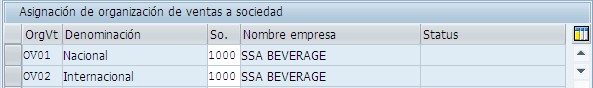
\includegraphics[scale=0.65,type=jpg,ext=.jpg,read=.jpg]{figures/OrgVentasSociedad}
\caption{Asignaci'on de las Organizaciones de Ventas a la Sociedad}
\label{fig:asigna1}
\end{figure}
\begin{figure}[htb]
\centering
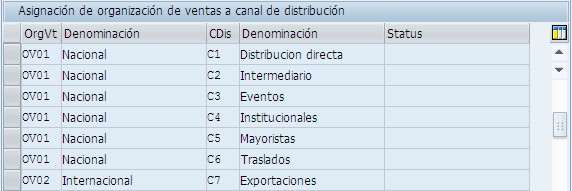
\includegraphics[scale=0.65,type=jpg,ext=.jpg,read=.jpg]{figures/OrgVentasCanales}
\caption{Asignaci'on de las Organizaciones de Ventas a los Canales de Distribuci'on}
\label{fig:asigna2}
\end{figure}
\begin{figure}[htb]
\centering
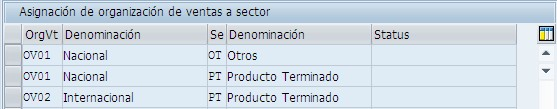
\includegraphics[scale=0.65,type=jpg,ext=.jpg,read=.jpg]{figures/OrgVentasSector}
\caption{Asignaci'on de las Organizaciones de Ventas a los Sectores}
\label{fig:asigna3}
\end{figure}
\begin{figure}[htb]
\centering
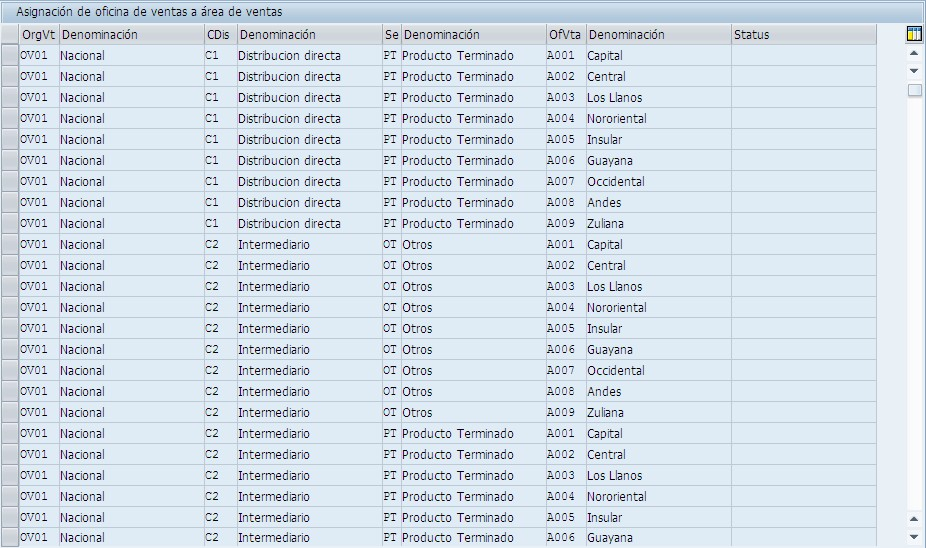
\includegraphics[scale=0.65,type=jpg,ext=.jpg,read=.jpg]{figures/OfVentaAreas}
\caption{Parte de la asignaci'on de las Oficinas de Ventas a las 'Areas de Ventas}
\label{fig:asigna4}
\end{figure}
\begin{figure}[htb]
\centering
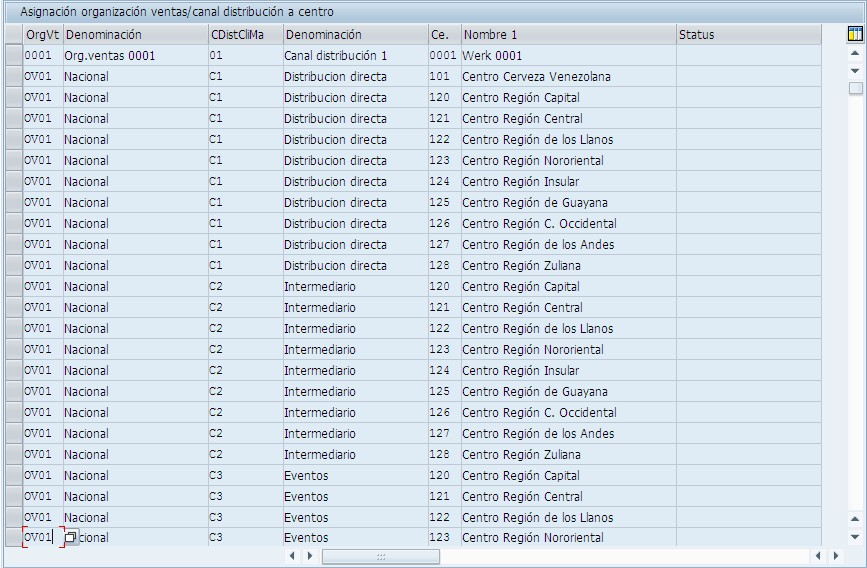
\includegraphics[scale=0.65,type=jpg,ext=.jpg,read=.jpg]{figures/OrgCanalCentro}
\caption{Parte de la asignaci'on de las Orgnanizaciones de Ventas y Canales de Distribuci'on a los Centros de Distribuci'on}
\label{fig:asigna5}
\end{figure}
\begin{figure}[htb]
\centering
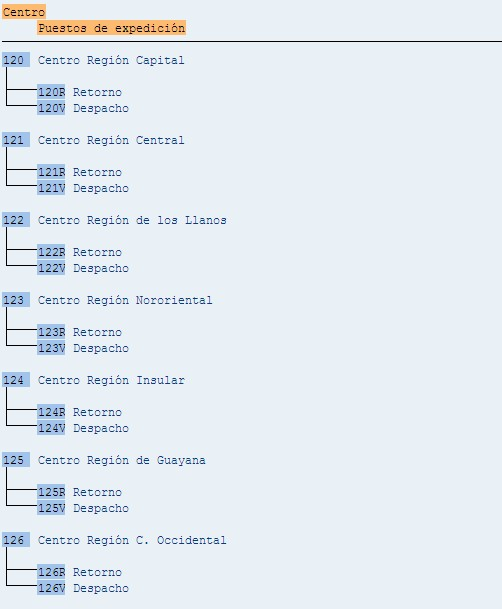
\includegraphics[scale=0.65,type=jpg,ext=.jpg,read=.jpg]{figures/ExpedicionCentro}
\caption{Parte de la asignaci'on de los Puestos de Expedici'on a los Centros de Distribuci'on}
\label{fig:asigna6}
\end{figure}

AQU\'I VA EL CONTENIDO DE LOS AP\'ENDICES.
%Puedes quitar esto(es opcional)
\vspace{5 mm}

Esta parte del ap'endice contiene el manual del usuario de la herramienta
implementada, la descripci'on de sus archivos y el c'odigo fuente de algunos
m'odulos de posible inter'es.

\section{Requerimientos de {\it software} y {\it hardware}}
\label{sect:hardsoftrequirements}

El programa resultante deber'ia poder ser utilizado sobre cualquier maquina 
con m'as de 32 MB libres de RAM. Aunque no hay limitaciones para el procesador
a usar, entre m'as nuevo el procesador y mayor n'umero de n'ucleos tenga, m'as
r'apido har'a los calculos la herramienta. En el caso de la memoria, entre 
m'as tenga disponible la herramienta, mayor cantidad de datos podr'a utilizar 
en los c'alculos.

\begin{itemize}
\item Para su compilaci'on, el programa requiere una versi'on actualizada de
gcc, el compilador {\tt C} GNU. Se ha utilizado varias versiones para su
compilaci'on por lo cualquier versi'on mayor a la $4.2$ deber'ia funcionar.
\item La liber'ia {\tt libpcap} es necesaria para darle las funcionalidades de
manipulaci'on de trazas {\tt tcpdump} al programa. A partir de la versi'on
$0.8$ se encuentran todas las funciones que utiliza el programa.
\item La compilaci'on de la herramienta se hace m'as f'acil con {\tt make},
programa GNU. Cualquier versi'on mayor a $3.6$ no deber'ia dar problemas.
\item El programa {\tt gnuplot} es indispensable para poder graficar los
resultados creados por el programa. La versi'on m'as utilizada durante su
desarrollo fue la $4.2$ por lo que es la que se recomienda.
\item La graficaci'on s'olo se puede hacer sobre un sistema operativo bajo el
est'andar POSIX\footnote{"Portable Operating System Interface [for Unix]" son
una familia de est'andares de llamadas al sistema operativo definidos por la
IEEE y especificados formalmente en el IEEE 1003. La gran mayor'ia de las
distribuciones GNU/Linux siguen los est'andares aunque no est'an
oficialmente certificados.} con la herramienta gnuplot instalada. Esto se debe
a una necesidad de la interfaz gnuplot en ANSI C que utiliza un ``pipe'' tipo
POSIX para comunicarse directamente con el programa gnuplot instalado en la
m'aquina. Sin embargo, dentro de las opciones del programa se puede pasar la
informaci'on obtenida en la estimaci'on a archivos de texto para su posterior
an'alisis.
\item La librer'ia pthreads da las funciones necesarias para utilizar hilos
de ejecuci'on en el programa.
\end{itemize}

\section{Ayuda de la l'inea de comando} \label{sect:ayuda}

La herramienta toma como par'ametro principal un archivo {\tt tcpdump} o un CSV
de una serie de tiempo pseudo-aleatoria generada con la herramienta R.
Aparte se puede escoger una velocidad de captura, una ventana, una ventana
deslizante, filtrar paquetes, delimitar corridas, correr con varios hilos de
ejecuci'on, adem'as de estimar el par'ametro de Hurst con los tres m'etodos
mencionados. Se puede tambi'en obtener el cambio del par'ametro de Hurst en el
tiempo o graficar la estimaci'on de una ventana en particular. La ayuda de la
l'inea de comando se muestra abajo:

\begin{alltt}
\label{verb:help}
Usage: ./d2Hgr -[f|g] file -[i|nrlvxmu] [OPTIONS]                               

Estimate and graph Hurst parameter calculations from a file.

   -f file   Specifies a tcpdump dump file.
   -g file   Specifies a CSV file with a simulated network traffic stream.
             This option cannot be used with the time based or tcpdump
             options since the stream is simulated and is static in it's
             definition.
   -i        Prints only the protocol statistic information available from the
             tcpdump file.
   -n        Tells the program if you wish to graph the packets per delta time
             graph. Affected by -p, -o, -d, -c, -b -e, -y flags.
   -r        Tells the program to calculate the Hurst parameter changes over
             time by use of the R/S statistic. Affected by -p, -o, -d, -c, -w,
             -s, -j, -t, -b, -e, -y flags.
   -l num    Tells the program to graph the Pox diagram that creates the Hurst
             data point for a given window number between 0 and Datapoints
             designated by num. Affected by -p, -o, -d, -c, -w, -s, -j, -b,
             -e, -y flags.
   -v        Tells the program to calculate the Hurst parameter changes over
             time by using the Variance-time plot technique. Affected by -p,
             -o, -d, -w, -s, -j, -t, -b, -e, -y flags.
   -x num    Tells the program to graph the Variance-time plot that estimates
             the Hurst parameter for a given window number designated by num.
             Affected by -p, -o, -d, -c, -w, -s, -j, -b, -e, -y flags.
   -m        Tells the program to calculate the Hurst parameter changes over
             time by use of the Modified Allan Variance. Affected by -p, -o,
             -d, -c, -w, -s, -j, -t, -b, -e, -y flags.
   -u num    Tells the program to graph the Modified Allan Variance that
             estimates the Hurst parameter for a given window number designated
             by num. Affected by -p, -o, -d, -c, -w, -s, -j, -t, -b, -e, -y
             flags.

 OPTIONS:
   -p proto  Specifies which protocol to be taken into account when doing
             calculations. Default is all.
             Implemented protocols are:
              ip tcp udp icmp sctp ftp ssh telnet smtp dns dhcp http pop3 ntp
              imap snmp ldap https smtps ldaps imaps pop3s nfs squid
   -o dir    Output directory for results. Default is current directory.
   -d        Tells the program if the results should be placed in text files
             for later use. This option doesn't graph. Useful for using this
             program where gnuplot is not available.
   -y        Tells the program to graph and print the resulting data files.
   -a        Tells the program not to graph or create data files.
   -c sec    Specify a packet capture speed. This makes the program not look
             for one. Example: 0.01 = 0.01 seconds.
   -w sec    Window time size. This makes the program not look for one.
             Example: 60 = 60 seconds.
   -s sec    Slide time size. This makes the program not look for one.
             Example: 1 = 1 seconds.
   -j num    Tells the program to use log base num for all the calculations of
             blocks for the R/S statistic, Variance-time plot and Modified Allan
             Variance. Default is 2.
   -t num    Does Hurst calculation using threads. If 0 is placed, then the
             default number of threads (4) is used.
   -b sec    Tells the program from which second in the time data to begin the
             calculation. Default is 0s.
   -e sec    Tells the program how many seconds after the beginning point to
             include in the calculation. Default is the whole tcpdump time.
   -k num    Average Hurst parameter change with which to try to detect attacks.
   -K num    Standard deviation of Hurst parameter change with which to detect
             attacks.
   -q num    Average Hurst parameter value with which to try to detect attacks.
   -Q num    Standard deviation of Hurst parameter value with which to detect
             attacks.
   -h        Print this help.
\end{alltt}

\section{Archivos del programa}

El programa de C llamado {\tt d2Hgr}, consiste de 18 archivos de c'odigo fuente
que incluye 9 archivos de cabecera. Los archivos contienen la siguiente
informaci'on:

\begin{itemize}
\item{\bf config.h}: Cabecera de funciones para parsear las opciones de linea
de comando.
\item{\bf config.c}: Implementaci'on de las funciones que parsean las opciones
de la linea de comando.
\item{\bf d2Hgr.h}: Archivo que contiene las definiciones de las funciones para
leer los archivos producidos por {\tt tcpdump}.
\item{\bf d2Hgr.c}: Implementaci'on de las funciones para leer la informaci'on
del archivo producido por {\tt tcpdump} y poder obtener la informaci'on
necesaria para su posterior an'alisis.
\item{\bf externvars.h}: Archivo que contiene todas las estructuras especiales
para el uso del programa.
\item{\bf filter.h}: Archivo que contiene la definici'on de las funciones para
construir la expresi'on de filtro de libpcap para usar durante la corrida del
programa.
\item{\bf filter.c}: Archivo que contiene la implementaci'on de todas las
funciones de filter.h.
\item{\bf flows.h}: Cabecera de funciones para contabilizar los flujos de IPv4.
\item{\bf flows.c}: Archivo que contiene la definici'on de las funciones para
contabilizar los flujos de IPv4.
\item{\bf gnuplot\_i.h}: Cabecera para el archivo gnuplot\_i.c que define las
funciones de la interfaz gnuplot para que el programa pueda graficar los
resultados. Esta es una versi'on modificada de la interfaz ANSI C de N.
Devillard para gnuplot.
\item{\bf gnuplot\_i.c}: Implementaci'on de las funciones de N. Devillard para
su interfaz de ANSI C con gnuplot.
\item{\bf graph.h}: Archivo que contiene la definici'on de las funciones para
graficar los resultados.
\item{\bf graph.c}: Archivo que contiene la implementaci'on de las funciones
para graficar los resultados.
\item{\bf hurst.h}: Archivo que contiene las definiciones de los m'etodos para
aproximar el par'ametro de Hurst.
\item{\bf hurst.c}: Archivos que contiene las implementaciones de los m'etodos
para aproximar el par'ametro de Hurst y los m'etodos para extraer la
informaci'on sobre los paquetes una vez leidos por las funciones de d2Hgr.h.
\item{\bf main.c}: El archivo que contiene el main del programa.
\item{\bf detect.h}: El archivo que contiene las definiciones de los m'etodos 
para la detecci'on de ataques de denegaci'on de servicio.
\item{\bf detect.c}: El archivo que contiene las implementaciones de los 
m'etodos para la detecci'on de ataques de denegaci'on de servicio.
\end{itemize}

\section{Creaci'on de $Xtdata$}

\lstinputlisting[caption={Creaci'on de $Xtdata$},label={cod:xtdata}]{code/xtdatacreate.c}



\chapter{Configuraciones Realizadas en el Proyecto}
\begin{table}[htb]
\footnotesize
\begin{tabular}{|c|}
\hline
\textbf{Configuraciones Realizadas}\\
\hline
Creaci'on de Organizaciones de Ventas, Canales de Distribuci'on y Sectores\\
\hline
Creaci'on de Oficinas de Ventas y 'Areas de Ventas\\
\hline
 Asignar las Organizaciones de Ventas creadas a la Sociedad\\
\hline
Asignar los Canales de Distribuci'on a las Organizaciones de Ventas\\
\hline
Asignar los Sectores a las Organizaciones de Ventas \\
\hline
Asignar las Oficinas de Ventas a las 'Areas de Ventas\\
\hline
Asignar las Organizaciones de Ventas y Canales de Distribuci'on a los Centros de Distribuci'on\\
\hline
Asignar los Puestos de Expedici'on a los Centros de Distribuci'on\\
\hline
\end{tabular}
\caption{Configuraciones realizadas para establecer la relaci'on entre las distintas unidades componentes de la estructura de SSA Beverage}
\label{tb:asignaciones}
\end{table}
\section{Configuraci'on de la Estructura de SSA Beverage}
	En esta secci'on se presentan las im'agenes de la estructura resultante de la segunda fase del desarrollo del proyecto.
\begin{figure}[H]
\centering
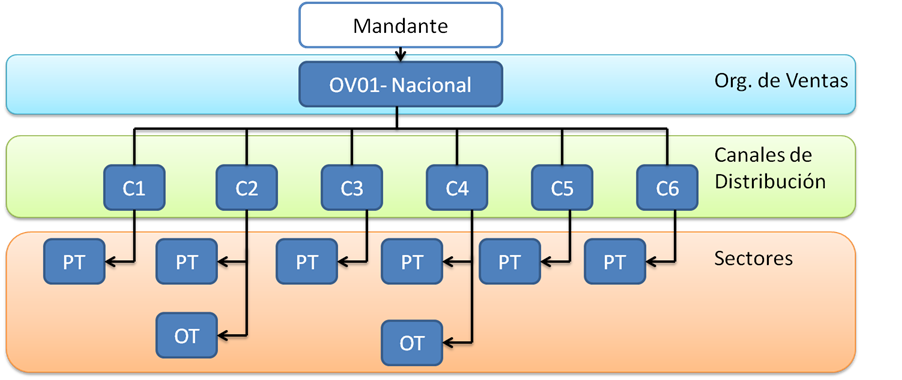
\includegraphics[scale=0.65,type=png,ext=.png,read=.png]{figures/Org1}
\caption{Estructura de SSA Beverage resultante de la Fase del Blueprint}
\label{fig:estructura1}
\end{figure}
\begin{figure}[H]
\centering
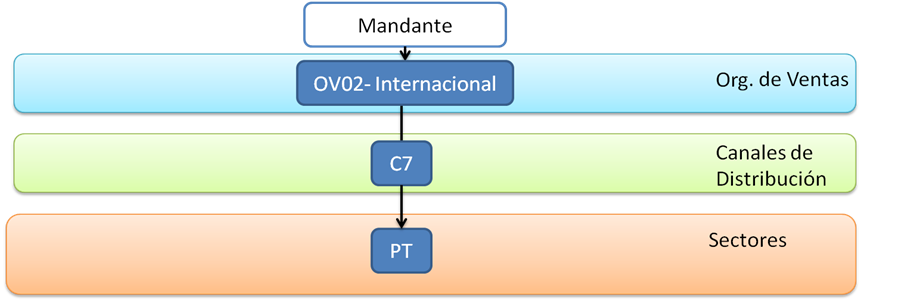
\includegraphics[scale=0.65,type=png,ext=.png,read=.png]{figures/Org2}
\caption{Estructura de SSA Beverage resultante de la Fase del Blueprint - Parte 2}
\label{fig:estructura2}
\end{figure}

	A continuaci'on, se muestra las configuraciones realizadas sobre la estructura de la empresa dentro de SAP SD.
	
	\subsection*{Creaci'on de las Organizaciones de Ventas}
\begin{figure}[H]
\centering
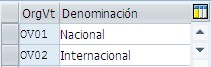
\includegraphics[scale=0.65,type=jpg,ext=.jpg,read=.jpg]{figures/OrgVentas}
\caption{Organizaciones de Ventas}
\label{fig:organizaciones}
\end{figure}

\subsection*{Creaci'on de los Canales de Distribuci'on}
\begin{figure}[H]
\centering
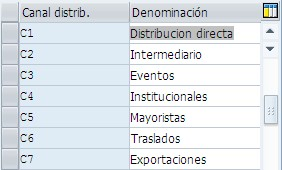
\includegraphics[scale=0.65,type=jpg,ext=.jpg,read=.jpg]{figures/CanalesDistribucion}
\caption{Canales de Distribuci'on}
\label{fig:canales}
\end{figure}

\subsection*{Creaci'on de los Sectores}
\begin{figure}[H]
\centering
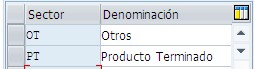
\includegraphics[scale=0.65,type=jpg,ext=.jpg,read=.jpg]{figures/Sectores}
\caption{Sectores}
\label{fig:sectores}
\end{figure}

\subsection*{Creaci'on de las 'Areas de Ventas}
\begin{figure}[H]
\centering
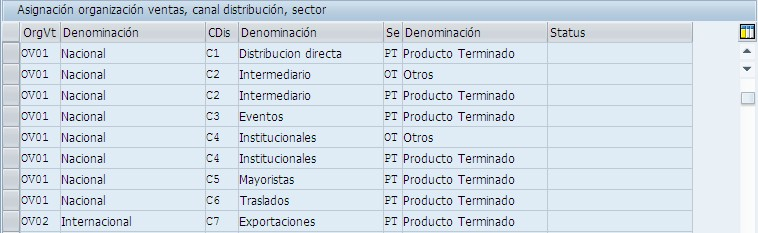
\includegraphics[scale=0.65,type=jpg,ext=.jpg,read=.jpg]{figures/AreaVentas}
\caption{'Areas de Ventas}
\label{fig:areas}
\end{figure}

\subsection*{Creaci'on de las Oficinas de Ventas}
\begin{figure}[H]
\centering
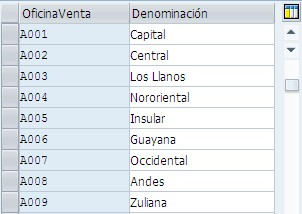
\includegraphics[scale=0.65,type=jpg,ext=.jpg,read=.jpg]{figures/OfVenta}
\caption{Oficinas de Ventas}
\label{fig:oficinas}
\end{figure}

\subsection*{Parte de la creaci'on de los Puestos de Carga}
\begin{figure}[htb]
\centering
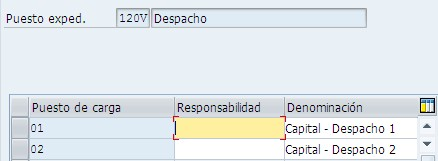
\includegraphics[scale=0.65,type=jpg,ext=.jpg,read=.jpg]{figures/PuestoCarga}
\caption{Parte de los Puestos de Carga definidos para el M'odulo SD}
\label{fig:carga}
\end{figure}

	En las configuraciones sucesivas de esta secci'on, lo que se realiz'o fue el establecimiento de las relaciones entre las distintas componentes de la empresa.

\subsection*{Asignaci'on de las Organizaciones de Venta a los Canales de Distribuci'on}	
\begin{figure}[H]
\centering
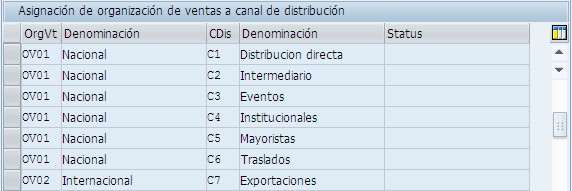
\includegraphics[scale=0.65,type=jpg,ext=.jpg,read=.jpg]{figures/OrgVentasCanales}
\caption{Asignaci'on de las Organizaciones de Ventas a los Canales de Distribuci'on}
\label{fig:asigna2}
\end{figure}

\subsection*{Asignaci'on de las Organizaciones de Ventas a los Sectores creados}
\begin{figure}[H]
\centering
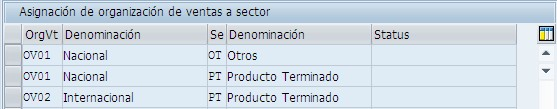
\includegraphics[scale=0.65,type=jpg,ext=.jpg,read=.jpg]{figures/OrgVentasSector}
\caption{Asignaci'on de las Organizaciones de Ventas a los Sectores}
\label{fig:asigna3}
\end{figure}

\subsection*{Asignaci'on de las Oficinas de Ventas a las 'Areas de Ventas}
\begin{figure}[H]
\centering
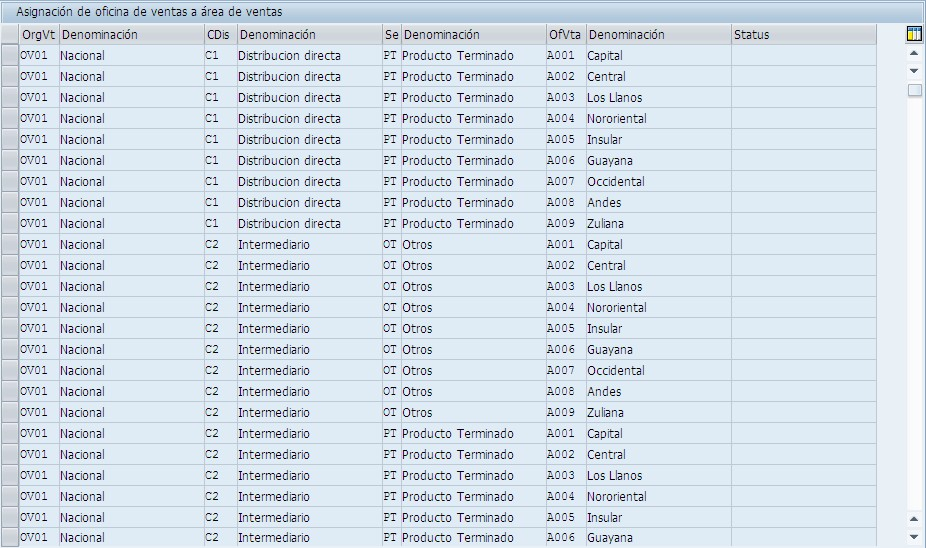
\includegraphics[scale=0.65,type=jpg,ext=.jpg,read=.jpg]{figures/OfVentaAreas}
\caption{Parte de la asignaci'on de las Oficinas de Ventas a las 'Areas de Ventas}
\label{fig:asigna4}
\end{figure}

\subsection*{Asignaci'on de las Organizaciones de Ventas y Canales de Distribuci'on a los Centros de Distribuci'on}
\begin{figure}[H]
\centering
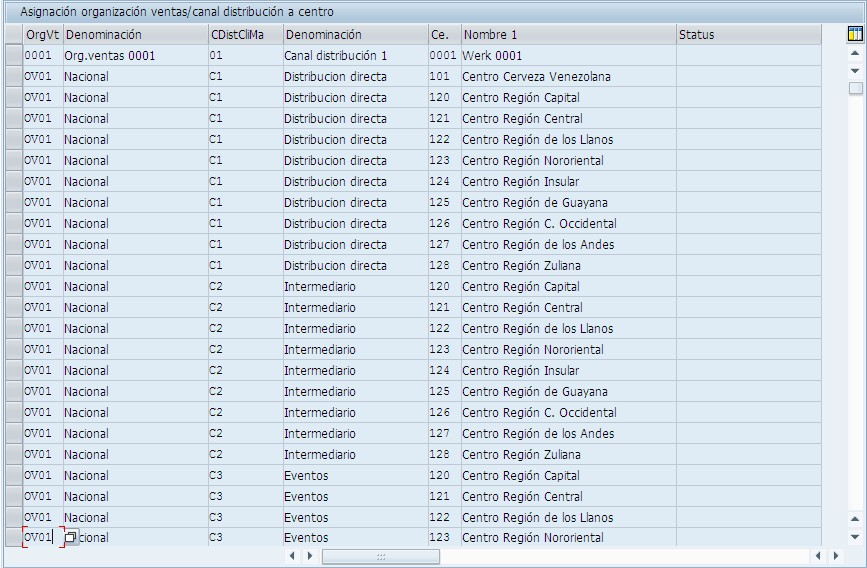
\includegraphics[scale=0.65,type=jpg,ext=.jpg,read=.jpg]{figures/OrgCanalCentro}
\caption{Parte de la asignaci'on de las Orgnanizaciones de Ventas y Canales de Distribuci'on a los Centros de Distribuci'on}
\label{fig:asigna5}
\end{figure}

\subsection*{Parte de la asignaci'on de los Puestos de Expedici'on a los Centros de Distribuci'on}
\begin{figure}[htb]
\centering
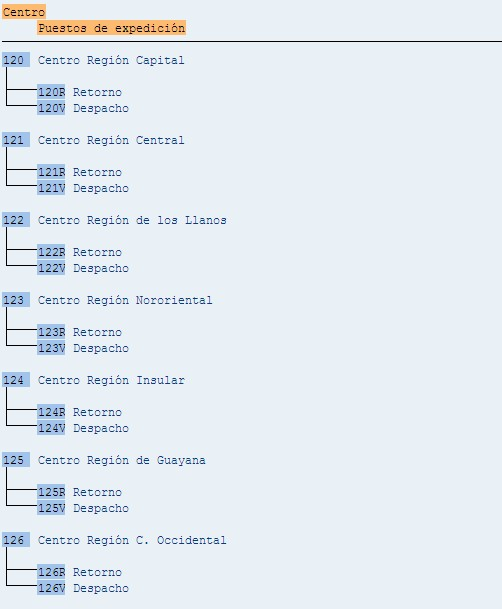
\includegraphics[scale=0.65,type=jpg,ext=.jpg,read=.jpg]{figures/ExpedicionCentro}
\caption{Parte de la asignaci'on de los Puestos de Expedici'on a los Centros de Distribuci'on}
\label{fig:asigna6}
\end{figure}

\chapter{Desarrollos realizados en ABAP/4}

\section{Programa de Carga Masiva de Datos del Maestro de Clientes}
\begin{figure}[H]
\centering
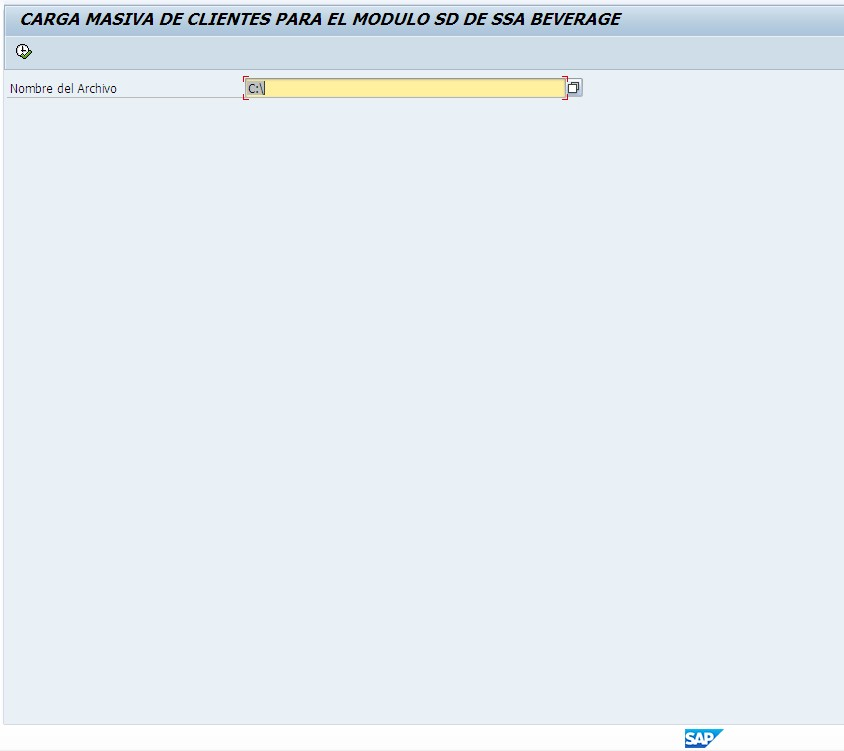
\includegraphics[scale=0.65,type=jpg,ext=.jpg,read=.jpg]{figures/screen}
\caption{Selection Screen para el Programa de Carga Masiva realizado}
\label{fig:screen}
\end{figure}

\begin{figure}[H]
\centering
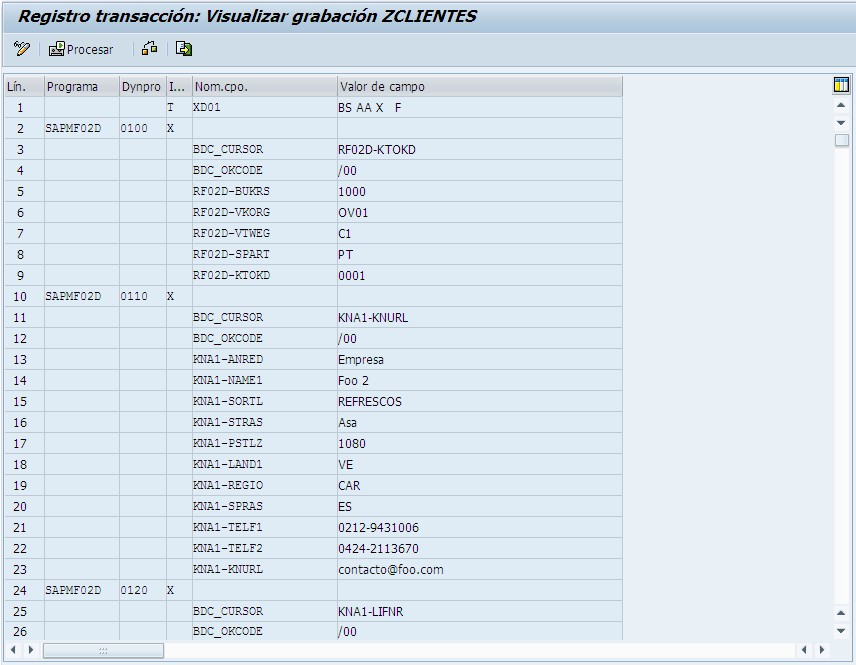
\includegraphics[scale=0.65,type=jpg,ext=.jpg,read=.jpg]{figures/sm35}
\caption{Grabaci'on realizada para la Carga Masiva}
\label{fig:sm35}
\end{figure}

\section{Creaci'on del Formulario de la Factura Legal}
\begin{figure}[H]
\centering
\begin{tabular}{c}
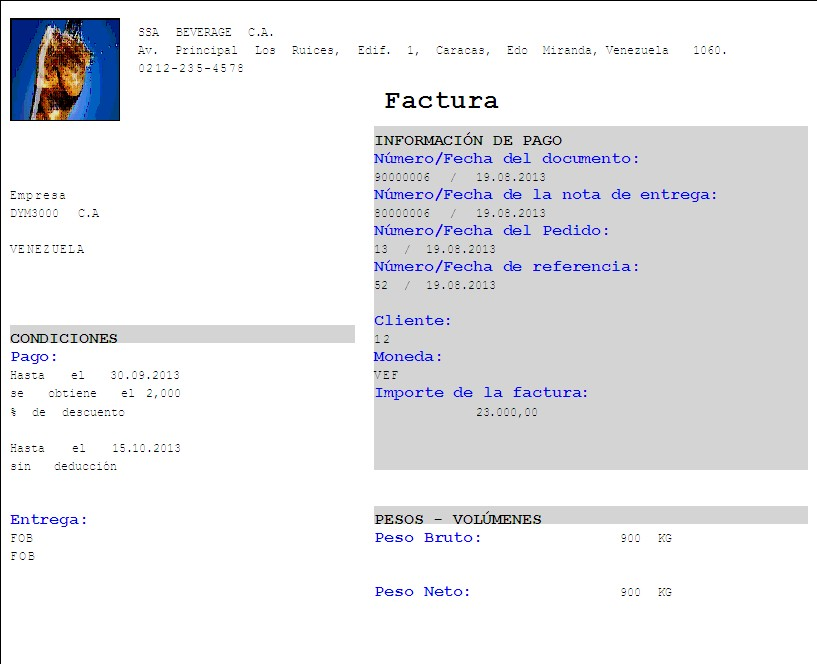
\includegraphics[scale=0.65,type=jpg,ext=.jpg,read=.jpg]{figures/Factura1}\\
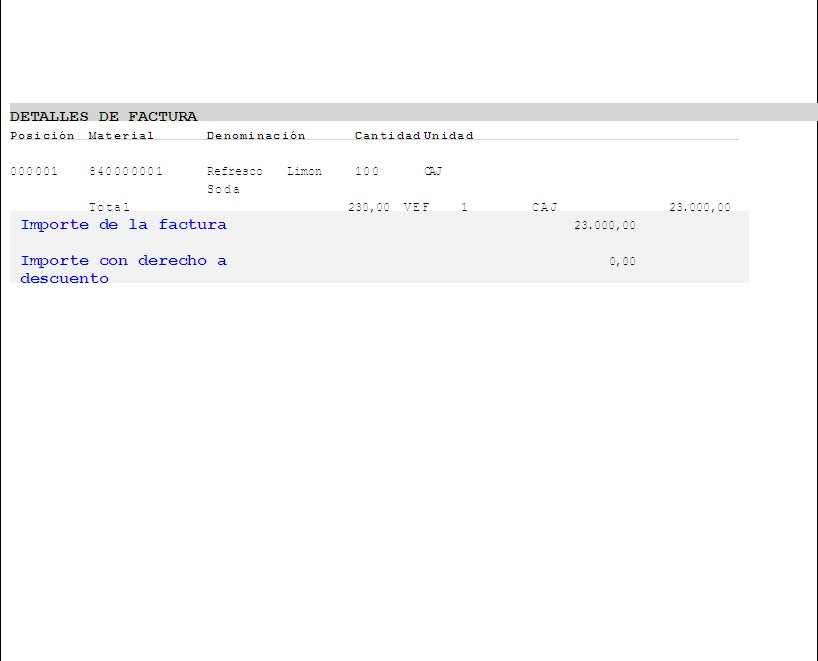
\includegraphics[scale=0.65,type=jpg,ext=.jpg,read=.jpg]{figures/Factura2}\\
\end{tabular}
\caption{Ejemplo de Factura creada para el m'odulo SD}
\label{fig:facturas}
\end{figure}

\section{Creaci'on de $Xtdata$}

\lstinputlisting[caption={Creaci'on de $Xtdata$},label={cod:xtdata}]{code/xtdatacreate.c}




\end{document}
